% В этом документе преамбула

%%% Работа с русским языком
\usepackage{cmap}					% поиск в PDF
\usepackage{mathtext} 				% русские буквы в формулах
\usepackage[T2A]{fontenc}			% кодировка
\usepackage[utf8]{inputenc}			% кодировка исходного текста
\usepackage[english,russian]{babel}	% локализация и переносы
\usepackage{indentfirst}			% чтобы первый абзац в разделе отбивался красной строкой
\frenchspacing						% тонкая настройка пробелов

%%% Приведение начертания букв и знаков к русской типографской традиции
\renewcommand{\epsilon}{\ensuremath{\varepsilon}}
\renewcommand{\phi}{\ensuremath{\varphi}}			% буквы "эпсилон"
\renewcommand{\kappa}{\ensuremath{\varkappa}}		% буквы "каппа"
\renewcommand{\le}{\ensuremath{\leqslant}}			% знак меньше или равно
\renewcommand{\leq}{\ensuremath{\leqslant}}			% знак меньше или равно
\renewcommand{\ge}{\ensuremath{\geqslant}}			% знак больше или равно
\renewcommand{\geq}{\ensuremath{\geqslant}}			% знак больше или равно
\renewcommand{\emptyset}{\varnothing}				% знак пустого множества

%%% Дополнительная работа с математикой
\usepackage{amsmath,amsfonts,amssymb,amsthm,mathtools} % AMS
\usepackage{icomma} % "Умная" запятая: $0,2$ --- число, $0, 2$ --- перечисление

%% Номера формул
\mathtoolsset{showonlyrefs=true} % Показывать номера только у тех формул, на которые есть \eqref{} в тексте.

%% Свои команды

% операции, не определённые (или имеющие иные обохначения) в мат. пакетах
\DeclareMathOperator{\sgn}{\mathop{sgn}}				% ф-ия sgn
\renewcommand{\tg}{\mathop{\mathrm{tg}}\nolimits}		% обозначение тангенса

%% Перенос знаков в формулах (по Львовскому)
\newcommand*{\hm}[1]{#1\nobreak\discretionary{}
{\hbox{$\mathsurround=0pt #1$}}{}}

%%% Работа с картинками
\usepackage{graphicx}  % Для вставки рисунков
\graphicspath{{images/}{images2/}}  % папки с картинками
\setlength\fboxsep{3pt} % Отступ рамки \fbox{} от рисунка
\setlength\fboxrule{1pt} % Толщина линий рамки \fbox{}
\usepackage{wrapfig} % Обтекание рисунков текстом

%%% Работа с таблицами
\usepackage{array,tabularx,tabulary,booktabs} % Дополнительная работа с таблицами
\usepackage{longtable}  % Длинные таблицы
\usepackage{multirow} % Слияние строк в таблице

%%% Теоремы
\theoremstyle{plain} % Это стиль по умолчанию, его можно не переопределять.
\newtheorem{theorem}{Теорема}[section]
\newtheorem{lemma}{Лемма}[section]
\newtheorem{definition}[theorem]{Определение}
\newtheorem{property}{Свойство}
 
\theoremstyle{definition} % "Определение"
\newtheorem{corollary}{Следствие}[theorem]
\newtheorem{exmp}{Пример}[section]
 
\theoremstyle{remark} % "Примечание"
\newtheorem*{nonum}{Решение}
\newtheorem*{evidence}{Доказательство}
\newtheorem*{remark}{Примечание}

%%% Программирование
\usepackage{etoolbox} % логические операторы

%%% Страница
\usepackage{extsizes} % Возможность сделать 14-й шрифт
\usepackage{geometry} % Простой способ задавать поля
	\geometry{top=25mm}
	\geometry{bottom=35mm}
	\geometry{left=35mm}
	\geometry{right=20mm}

%\usepackage{fancyhdr} % Колонтитулы
% 	\pagestyle{fancy}
 	%\renewcommand{\headrulewidth}{0pt}  % Толщина линейки, отчеркивающей верхний колонтитул
% 	\lfoot{Нижний левый}
% 	\rfoot{Нижний правый}
% 	\rhead{Верхний правый}
% 	\chead{Верхний в центре}
% 	\lhead{Верхний левый}
%	\cfoot{Нижний в центре} % По умолчанию здесь номер страницы

\usepackage{setspace} % Интерлиньяж (межстрочные интервалы)
%\onehalfspacing % Интерлиньяж 1.5
%\doublespacing % Интерлиньяж 2
%\singlespacing % Интерлиньяж 1

\usepackage{lastpage} % Узнать, сколько всего страниц в документе.

\usepackage{soulutf8} % Модификаторы начертания

\usepackage{hyperref}
\usepackage[usenames,dvipsnames,svgnames,table,rgb]{xcolor}
\hypersetup{				% Гиперссылки
    unicode=true,           % русские буквы в раздела PDF
    pdftitle={Заголовок},   % Заголовок
    pdfauthor={Автор},      % Автор
    pdfsubject={Тема},      % Тема
    pdfcreator={Создатель}, % Создатель
    pdfproducer={Производитель}, % Производитель
    pdfkeywords={keyword1} {key2} {key3}, % Ключевые слова
    colorlinks=true,       	% false: ссылки в рамках; true: цветные ссылки
    linkcolor=MidnightBlue,          % внутренние ссылки
    citecolor=black,        % на библиографию
    filecolor=magenta,      % на файлы
    urlcolor=blue           % на URL
}

\usepackage{csquotes} % Еще инструменты для ссылок

%\usepackage[style=authoryear,maxcitenames=2,backend=biber,sorting=nty]{biblatex}

\usepackage{multicol} % Несколько колонок

%%% Работа с графикой
\usepackage{tikz}
\usetikzlibrary{calc}
\usepackage{tkz-euclide}
\usetikzlibrary{arrows}
\usepackage{pgfplots}
\usepackage{pgfplotstable}

%%% Настройка подписей к плавающим объектам
\usepackage{floatrow}	% размещение
\usepackage{caption}	% начертание
\captionsetup[figure]{labelfont=bf,textfont=it,font=footnotesize}	% нумерация и надпись курсивом
% для подфигур: заголовок подписи полужирный, текст заголовка обычный
% выравнивание является неровным (т.е. выровненным по левому краю)
% singlelinecheck = off означает, что настройка выравнивания используется, даже если заголовок имеет длину только одну строку.
% если singlelinecheck = on, то заголовок всегда центрируется, когда заголовок состоит только из одной строки.
\captionsetup[subfigure]{labelfont=bf,textfont=normalfont,singlelinecheck=off,justification=raggedright}

%%% Stuff для графиков и рисунков



\begin{document}

\textit{Почаев Никита Алексеевич, гр. 8381}

\section*{Независимые эксперименты. (ДЗ на 14.03.20)}

\subsection*{Задача 1.}

Техническая система из $n$ блоков. Вероятность неисправности каждого блока - $p$. Имеется 2 комплекта блоков. Систему можно собирать 2-мя способами: 
\begin{enumerate}
	\item Спаять и проверить - работает или нет (распаять нельзя);
	\item Проверять каждый блок и в зависимости от того, работает или нет, вставлять его в систему. Тот блок, на который заменили, также необходимо проверять. Два блока одного типа оказались неисправными $\Rightarrow$ систему собрать невозможно.
\end{enumerate}
Найти вероятности: $P(A) = ?$, где событие $A$ - из имеющихся блоков получится собрать работающую систему.

\textit{Решение:}

\textbf{Рассмотрим способ \RNumb{1}.}

По условию задачи имеем 2 комплекта деталей $\Rightarrow$ при неисправности одной собранной схемы можно собрать вторую.

Событие $B_j$ - из $i$-го комплекта деталей можно собрать работающую систему. Событие $B_{jk}$ - $k$-ый элемент $j$-ого набора исправен, данный события независимы. По условию неисправность каждого блока - независимые в совокупности события. Следовательно,
\[ B_j = \bigcap\limits_{k=1}^{n} B_{jk} = \prod_{k=1}^{n} P(B_{jk}) = (1-p)^n \]

\[ A = B_1 \cup B_2 \Rightarrow P(A) = 1 - P(\bar B_1 \cup \bar B_2) = 1 - \prod_{k=1}^2 (1 - P(B_{jk})) = 1 - (1 - (1-p)^n)^2 \]

\textbf{Рассмотрим способ \RNumb{2}.}

Имеется возможность на этапе сборки заменить неисправный блок на исправный. Событие $C_l$ - имеется $l$-ый исправный блок в одном из комплектов. Пусть события $C_{l1}$ и $C_{l1}$ - исправен $l$-ый блок из 1/2 набора соотвественно.
\[ C_l = C_{l1} \cup C_{l2} \Rightarrow P(C_l) = 1 - P(\bar C_{l1} \cup \bar C_{l2}) = 1 - \sum_{m=1}^{2} (1-P(C_{lm})) = 1 - p^2 \]

В данном случае событие $A \eq$ удалось найти хотя бы по одному исправному блоку каждого типа, чтобы собрать схему.
\[ A = \bigcap\limits_{l=1}^n C_l; P(A) = \prod_{l=1}^{n} P(B_l) = (1-p^2)^n \]

Для наглядности выявления более выгодной формулы возьмём $p=0.4$ и построим соответствующие графики. Зелёным на графике обозначен 1-ый способ, а синим - 2-ой. Как видно, проверка каждого блока является предпочтительным способом сборки.
\begin{figure}[H]
	\center{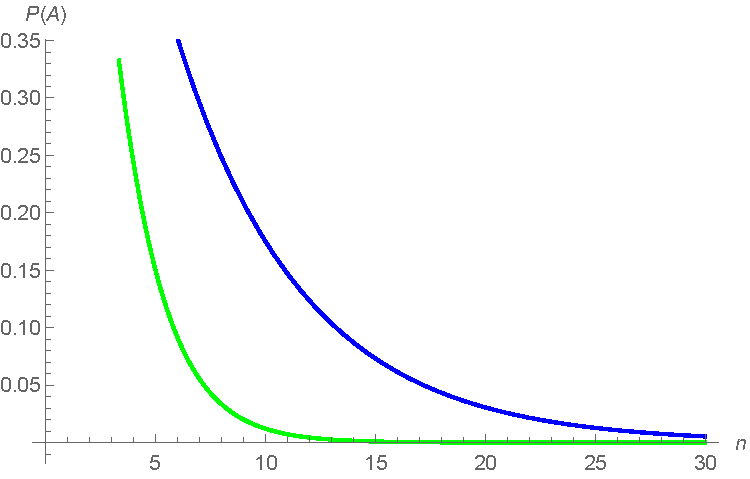
\includegraphics[scale=0.9]{./media/Homework-14-03-20_4.pdf}}
\end{figure}

\subsection*{Задача 2.}

Вероятность разрыва верёвки длины $l = 1$ равна $p$. Определить вероятность разрыва верёвки длины $L$, если разрыв непересекающихся участков верёвки происходит независимо.

\textit{Решение:}

Событие $A$ - верёвка разорвалась. Событие $B_i$ - разорвался $i$-ый участок верёвки. По условию задачи данные события независимы, поэтому:
\[ A = \bigcup\limits_{i=1}^{L} B_i \]

\[ P(A) = 1 - \prod_{i=1}^{L} (\bar B_i) = 1 - (1 - p)^{L} \]

\subsection*{Задача 3.}

Дана схема:
\begin{figure}[H]
	\center{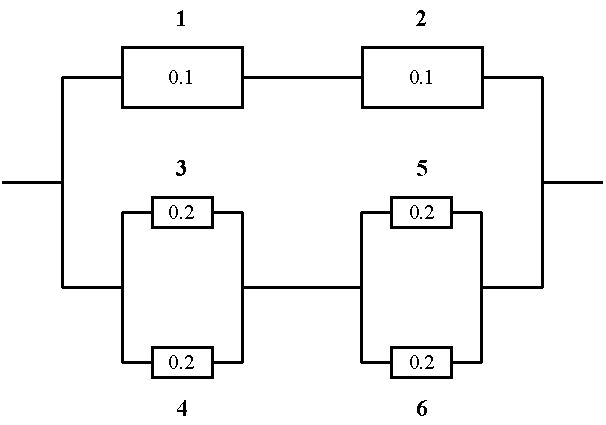
\includegraphics[scale=0.9]{./media/Homework-14-03-20_1.pdf}}
\end{figure}

Это механизм дублирования: отказывает один из верхних блоков $\to$ переходим на 2-ю ветку. Вероятность отказа каждого блока указана внутри. Событие $X$ - схема НЕ работает. Найти вероятность отказа системы $P(A) = ?$

\textit{Решение:}
\begin{align*}
\fbox{%
	\parbox{10cm}{%
		При нахождении веротности корректной работы последовательному соединению соответствует произведение событий, параллельному соединению - сумма событий. При нахождении веротности отказа системы наоборот.}%
}
\end{align*}

Ради удобства занумеруем элементы схемы, а находящиеся в одних группах (имеют одинаковое соединение) красим в один цвет.
\begin{figure}[H]
	\center{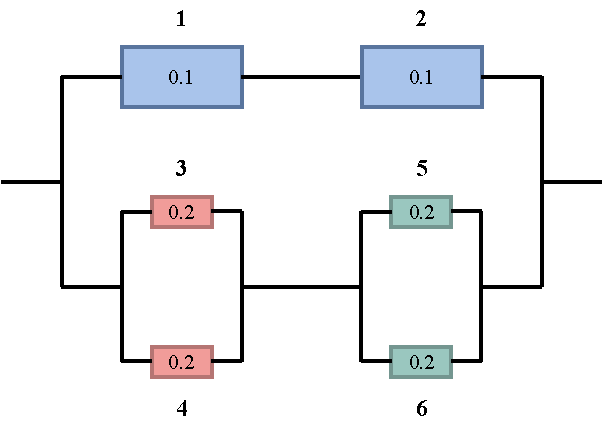
\includegraphics[scale=0.9]{./media/Homework-14-03-20_1_1.pdf}}
\end{figure}

\begin{itemize}
	\item 1 и 2 эл. - синий - последовательное соединения;
	\item 3 и 4 эл. - красный - параллельное соединения;
	\item 5 и 6 эл. - зелёный - параллельное соединения.
\end{itemize}

Событие $A_1$ - отказала синяя группа, $A_2$ - отказала красная группа, $A_3$ - отказала зелёная группа.

~

События:
\begin{itemize}
	\item $X_1$ - НЕ работает первый уровень схемы: синяя группа,
	\item $X_2$ - НЕ работает второй уровень схемы: красная и зелёная группы,
\end{itemize}

Пусть события $B_i$ - не работает $i$-ый блок в данной схеме.

$A_1 = B_1 \cup B_2$. Т.к. это единственная группа на первом уровне цепи, то вероятность его отказа равна $X_1 = A_1$.

\[ A_2 = B_3 \cap B_4 \]
\[ A_3 = B_5 \cap B_6 \]

Тогда вероятность отказа второго уровня цепи равна: $ X_2 = A_2 \cup A_3 = (B_3 \cap B_4) \cup (B_5 \cap B_6)$.

\[ X = X_1 \cap X_2 = (B_1 \cup B_2) \cap ((B_3 \cap B_4) \cup (B_5 \cap B_6)) \]

\[ P(X) = P((B_1 + B_2) \cdot ((B_3 \cdot B_4) + (B_5 \cdot B_6))) = \]
\[ = P(B_1 + B_2) \cdot P((B_3 \cdot B_4) + (B_5 \cdot B_6)) = \]
\[ = (P(B_1) + P(B_2) - P(B_1) \cdot P(B_2)) \cdot (P(B_3) \cdot P(B_4) + P(B_5) \cdot P(B_6) - P(B_3) \cdot P(B_4) \cdot P(B_5) \cdot P(B_6)) = \]
\[ = (0.1 + 0.1 - 0.1^2) \cdot (0.2^2 + 0.2^2 - 0.2^4) = 0.014896S \]

\subsection*{Задача 4.}

Дана схема, представленная на рисунке ниже.

Вероятность разрыва звена: $p_{\text{рз}} = p$. Событие $A$ - цепь разорвётся. Найти вероятность $P(A) = ?$
\begin{figure}[H]
	\center{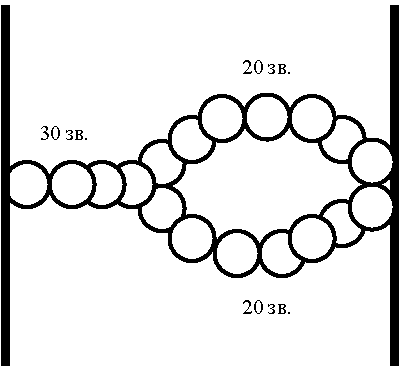
\includegraphics[scale=0.9]{./media/Homework-14-03-20_2.pdf}}
\end{figure}

\textit{Решение:}

Событие $B$ - разорвётся 1-ая часть цепи, состоящая из 30 звеньев. Событие $B_i$ - разорвётся $i$-ое звено.
\[ B = \bigcup\limits_{i=1}^{30} B_i \Rightarrow P(B) = 1 - \prod_{i=1}^{30}P(\bar B_i) = 1 - (1 - p)^{30} \]

Событие $C$ - разорвётся вторая часть цепи из двух хвостов (по 20 звеньев). События $C_u$ и $C_d$ - разорвётся верхняя (up) / нижняя (down) её часть. События $C_{uj}, C_{dk}$ - разорвётся соотвественно $j$-ое / $k$-ое звено частей данных цепей. Тогда:
\[ C_u = \bigcup\limits_{j=1}^{20} C_{uj} \Rightarrow P(C_u) = 1 - \prod_{j=1}^{20} (\bar C_{uj}) = 1 - (1 - p)^{20} \]

\[ C_d = \bigcup\limits_{k=1}^{20} C_{dk} \Rightarrow P(C_d) = 1 - \prod_{k=1}^{20} (\bar C_{dk}) = 1 - (1 - p)^{20} \]

Таким образов, вероятность события $C$ разорвалась верхняя И нижняя части цепи:
\[ C = C_u \cap C_d \Rightarrow P(C) = P(C_u) \cdot P(C_d) = (1 - (1 - p)^{20})^2 \]

Событие $A$ - разобрался первый участок цепи ИЛИ второй участок цепи.
\[ A = B \cup C \Rightarrow P(A) = 1 - ((1 - p)^{30} \cdot (1 - (1 - (1 - p)^{20})^2)) \]

\subsection*{Задача 5.}

Дана следующая схема электропередач. Вероятность повреждения ураганом линий передач между ними равна соответствующим числам. Определить вероятность $P$, что в пункте $C$ будет нарушено электроснабжение. Ток идёт из станции $A$. Будем считать, что отказ линии электропередач происходит независимо.
\begin{figure}[H]
	\center{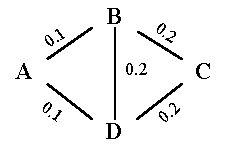
\includegraphics[scale=1.4]{./media/Homework-14-03-20_3.pdf}}
\end{figure}

\textit{Решение:}

Обозначим величины вероятности вероятности выхода из строя передач за $p = 0.1$ и $q = 0.2$. 

Событие $D$ - нарушено электроснабжение из $A$ в $C$.

Событие $A_B$ - нарушено электроснабжение из $A$ по пути $AB$ и только по нему.

Аналогично событие $B_C$ - нарушено электроснабжение по $BC$.

Событие $B_{DC}$ - нарушено электроснабжение по пути $BD - DC$.

\[ P(A_B) = p \cdot (1 - p) = 0.1 \cdot (1 - 0.1) = 0.09 \]
\[ P(B_C) = q = 0.2 \]
\[ P(B_{DC}) = 1 - (1 - q)^2 = 0.36 \]
\[ P(D|A_B) = P(B_C) \cdot P(B_{DC}) = 0.2 \cdot 0.36 = 0.072 \]
\[ P(DA_B) = P(D|A_B) \cdot P(A_B) = 0.00648 \]

Событие $A_D$ - нарушено электроснабжение из $A$ по пути $AD$ и только по нему.

Событие $D_C$ - нарушено электроснабжение по пути $DC$.

Событие $D_{BC}$ - нарушено электроснабжение по пути $DB - BC$.

\[ P(A_D) = P(A_B) \]
\[ P(D_C) = P(B_C) \]
\[ P(D_{BC}) = P(B_{DC}) \]

\[ P(DA_D) = P(DA_B) = 0.00648 \]

Событие $A_0$ - не нарушен ни один из путей из $A$, тогда:
\[ P(A_0) = (1 - p)^2 = 0.81 \]
\[ P(D|A_0) = P(D_C) \cdot P(B_C) = 0.04 \]
\[ P(DA_0) = 0.81 \cdot 0.04 = 0.0324 \]

Событие $A_{BD}$ - нарушено электроснабжение по обоим путям, тогда:
\[ P(D) = P(DA_B) + P(DA_D) + P(DA_0) +P(DA_{BD}) = 0.05536 \]

\end{document} 